\documentclass{beamer}
\usepackage{tikz}
\usepackage{float}
\usepackage{graphicx}
\usepackage[most]{tcolorbox}
\usetikzlibrary{decorations.pathreplacing}
\tcbuselibrary{theorems}
\tcbset{enhanced,colframe=blue!20,colback={black!5!white},drop shadow}
\setbeamertemplate{section in toc}[sections numbered]
\setbeamertemplate{subsection in toc}[subsections numbered]
\usetheme[numbering=fraction]{metropolis}           % Use metropolis theme
\title{Bachelor Thesis Marginal-Sampling}
\date{28.05.2020}
\author{Michael Fedders}

\newcommand{\s}{\sigma^2}
\newcommand{\sh}{\hat{\sigma}^2}
\begin{document}
	\maketitle
  	\begin{frame}[plain]
		\frametitle{Table of Contents}
		\tableofcontents
	\end{frame}
	
\section{Introduction / Motivation}

  	\begin{frame}{Motivation}
	  	In the area of applied mathematics and especially while we are working
	  	with model based assumptions we have to deal with uncertainties. Mainly
	  	there are two possible points:
	  	\begin{itemize}
	  		\item during observation of the model there may be a \alert{loss} of 
	  		dimension
	  		\item measuring variables can add a \alert{noise}
	  	\end{itemize}
	\end{frame}
  
  	\begin{frame}{Mathmatical model}
     	In this setting we will focus on ODE models. The original model can be described
     	through
     	\[
     	\frac{dx(t,\theta)}{dt} = f(x(t,\theta),\theta), \quad x(t_0,\theta) = 
     	x_0(\theta)
     	\]
     	with $x$ as our state vector, $t$ as the time and $\theta$ representing
     	parameters from our system, which are unknown at the start.
	\end{frame}
	
	\begin{frame}{Observation function}
  		We can not analyse the function directly but have to use
		\[
			y(t_k,\theta) = \tilde{h}(h(x(t_k,\theta),\theta))
		\]
		and, assuming additive noise
		\[
			\overline{y}_{k} = y(t_k,\theta) + \epsilon_{k}
		\]
	\end{frame}
	
	
  	\begin{frame}{Measure uncertainties}
    	We can group this data observation in three steps.      	
  	\end{frame}
  	
  	\begin{frame}{Measure uncertainties}
    	We can group the data interpretation in three steps.
  		\begin{itemize}
   			\item observation function $h(x(t_k,\theta))$
    	\end{itemize}
  	\end{frame}
  	
  	\begin{frame}{Measure uncertainties}
    	We can group the data interpretation in three steps.
    	\begin{itemize}
    		\item observation function $h(x(t_k,\theta))$
    		\item relative experimental data through $y_k = \tilde{h}
    		(h(t_k, \theta))$
    	\end{itemize}
  	\end{frame}
  	
  	\begin{frame}{Measure uncertainties}
    	We can group the data interpretation in three steps.
    	\begin{itemize}
    		\item observation function $h(x(t_k,\theta))$
    		\item relative information $y_k = \tilde{h}
    		(h(t_k, \theta))$
    	\end{itemize}
    	For example:
    	\vspace{0.7cm}
    	\begin{columns}
  			\begin{column}{5cm}
  				$y(t_k,\theta,c) = c + h(x(t_k,\theta),\theta)$
  			\end{column}
  			\begin{column}{5cm}
 				$y(t_k,\theta,s) = s \cdot h(x(t_k,\theta),\theta)$
  			\end{column}
  		\end{columns}
  	\end{frame}
  	
  	\begin{frame}{Measure uncertainties}
    	We can group the data interpretation in three steps.
    	\begin{itemize}
    		\item observation function $h(x(t_k,\theta))$
    		\item relative information $y_k = \tilde{h}
    		(h(t_k, \theta))$
    	\end{itemize}
    	For example:
    	\vspace{0.7cm}
    	\tcbox[colframe=red!75!black]
  		{$y(t_k,\theta,c) = c + h(x(t_k,\theta),\theta)$}
  	\end{frame}  	
  	
  	\begin{frame}{Measure uncertainties}
    	We can group the data interpretation in three steps.
    	\begin{itemize}
    		\item observation function $h(x(t_k,\theta))$
    		\item relative experimental data through $y_k = \tilde{h}
    		(h(x(t_k,\theta)))$
    		\item adding the noise $\overline{y}_{k} = y + \varepsilon_{k}$
    	\end{itemize}
  	\end{frame}
  	
  	\begin{frame}{Measure uncertainties}
    	We can group the data interpretation in three steps.
    	\begin{itemize}
    		\item observation function $h(x(t_k,\theta))$
    		\item relative experimental data through $y = \tilde{h}
    		(h(x(t_k,\theta))$
    		\item adding the noise $\overline{y}_{k} = y + \varepsilon_{k}$
    	\end{itemize}
    	For example:
    	\vspace{0.7cm}
    	\begin{columns}
  			\begin{column}{3cm}
  				$\varepsilon_{k} \sim \mathcal{N}(0,\s)$
  			\end{column}
  			\begin{column}{4cm}
 				$\varepsilon_{k} \sim \operatorname{Laplace}(0,\sigma)$
  			\end{column}
  		\end{columns}
  	\end{frame}
  	
  	\begin{frame}{Measure uncertainties}
    	We can group the data interpretation in three steps.
    	\begin{itemize}
    		\item observation function $h(x(t_k,\theta))$
    		\item relative experimental data through $y = \tilde{h}
    		(h(x(t_k,\theta))$
    		\item adding the noise $\overline{y}_{k} = y + \varepsilon_{k}$
    	\end{itemize}
    	For example:
    	\vspace{0.7cm}
  		\tcbox[colframe=red!75!black]
  		{$\epsilon_{k} \sim \mathcal{N}(0,\s)$}
  	\end{frame}
  	
  	\begin{frame}{Measure uncertainties}
    	We can group the data interpretation in three steps.
    	\begin{itemize}
    		\item observation function $h(x(t_k,\theta))$
    		\item relative experimental data through $y = \tilde{h}
    		(h(x(t_k,\theta))$
    		\item adding the noise $\overline{y}_{k} = y + \varepsilon_{k}$
    	\end{itemize}
    	In total we get:
    	\vspace{0.7cm}
  		\tcbox[colframe=red!75!black]
  		{$\overline{y}_{k} = c + (h(x(t_k,\theta)) + \varepsilon_{k}$ with $
  		\varepsilon_k \sim \mathcal{N}(0, \s)$}
  	\end{frame}
     
  	\begin{frame}{Bayes Theorem}
  		We now want to use data to estimate our parameters. To 
  		do so we will use Bayes Theorem: %(formula for normal)
  	\end{frame}

	\begin{frame}{Bayes Theorem}
  		We now want to use data to estimate our parameters. To 
  		do so we will use Bayes Theorem:
  		\[  \tcboxmath{p(\theta,c,\s \mid D) = \frac{p(D \mid \theta,c,\s) \cdot
  		p(\theta) \, p(c) \, p(\s)}{p(D)}} \]
  	\end{frame}
  	
	\begin{frame}{Marginalization of the posterior}
  		But from a process standpoint we are only 
  		interested in the distribution of $\theta$ and therefore would like to 
  		only calculate $p(\theta \mid D)$ which has less dimensions to be sampled.
  	\end{frame}
  	
  	\begin{frame}{Marginalization of the posterior}
		To get this result we take the expected value from both sides over the 
		parameters introduced by the noise $\varepsilon$ and the relative factor 
		$\tilde{h}$ and receive:
		\[
			p(\theta \mid D) = \frac{p(D \mid \theta) \cdot p(\theta)}{p(D)}
		\]
		with 
		\[
			p(D \mid \theta) = \int_{\mathbb{R}_+} \int_{\mathbb{R}} p(D \mid 
			\theta,c,\s) p(c) p(\s) \, dc \, d\s
		\]
  	\end{frame}  
  
\section{Personal progress}
	
	\begin{frame}{Calculation}
		By inserting the likelihood function we receive
		\[
			\int_{\mathbb{R}_+} \int_\mathbb{R} \prod_{k = 1}^N \frac{1}{\sqrt{2 
			\pi \s}} \exp\left(-\frac{1}{2} \left(\frac{\overline{y}_{k} -\left( c 
			+ h_{k} \right)}{\sigma} \right)^2\right) \, p(c) \, p(\s) \, dc 
			\, d\s
		\]
	\end{frame}


	\begin{frame}{Choice of priors}
		One main choice here is, which priors $p(c)$ and $p(\s)$ we use, as they 
		are defining the distribution of $c$ and $\s$.
	\end{frame}

	\begin{frame}{Choice of priors}
		First choice: "flat" priors, aka $p(c) = p(\s) = 1$. The problem with this
		choice is, that
		\[
			\int_\mathbb{R} 1 \, dx = \infty \neq 1
		\]
		so we are not using a probability distribution here.
	\end{frame}

	\begin{frame}{Choice of priors}
		First choice: "flat" priors, aka $p(c) = p(\s) = 1$. The problem with this
		choice is, that
		\[
			\int_\mathbb{R} 1 \, dx = \infty \neq 1
		\]
		so we are not using a probability distribution here.
	
		\vspace{1cm}
		\alert{But}: We can still argue, that this choice is preserving enough 
		information to make it a valid first choice.
	\end{frame}

	\begin{frame}{Calculation}
		If we now insert $p(c) = p(\s) = 1$ in
		\[
			\int_{\mathbb{R}_+} \int_\mathbb{R} \prod_{k = 1}^N \frac{1}{\sqrt{2 \pi \s}} \exp\left(-\frac{1}{2} 
			\left(\frac{\overline{y}_{k} -\left( c + h_{k} \right)}{\sigma}
		 	\right)^2\right) \, p(c) \, p(\s) \, dc \, d\s
		\]
		we can substitute twice and get
		\[
			\frac{\bigl(\sqrt{N}\bigr)^{N-4}}{2\bigl(\sqrt{\pi}\bigr)^{N-1}} \cdot 
			\Biggl(N \cdot \sum_{k = 1}^N (h_k - \overline{y_k})^2 - \Biggl
			(\sum_{k = 1}^N \overline{y_k} - h_k)\Biggr)^2 \ \Biggr)^{-(N-3)/2} 
			\cdot \Gamma \biggl(\frac{N-3}{2}\biggr)
		\]
	\end{frame}

	\begin{frame}{Numerical testing}
		First test with basic sample regression model:
		\begin{itemize}
			\item $y(t,\theta,c) = c + t$ and
			\item $t_k = k$
		\end{itemize}
		In total we get $\overline{y}_k \sim \mathcal{N}(c + t_k,\s)$.
	\end{frame}

	\begin{frame}{Plot}
		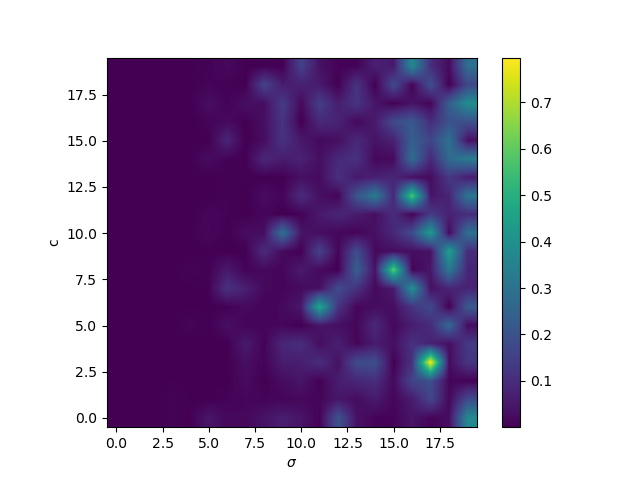
\includegraphics[scale=0.8]{heatmap.png}
	\end{frame}

\section{Next steps}

	\begin{frame}{Current work}
		\begin{itemize}
			\item The next steps for the flat prior choice will be to implement 
			test examples of ODEs to further test the analytical derivation.
			\item I also started the calculation of the integral in the case of a 
			gaussian prior $c  \sim \mathcal{N}(\mu, \hat{\sigma}^2)$.
		\end{itemize}
	\end{frame}

	\begin{frame}{Gaussian prior}
		By defining three constants
		\[
			K_1 = \biggl(\sum_{k = 1}^N (\overline{y_k} - h_k) \biggr)^2, \ K_2 
			= \sum_{k = 1}^N (\overline{y_k} - h_k)^2, \ K_3 = 
			\sum_{k = 1}^N (\overline{y_k} - h_k)
		\]
		we can rewrite the integral in the following way:
	\end{frame}

	\begin{frame}{Gaussian prior}
		\[
    		\int_0^{\infty} \frac{1}{(2\pi\s)^{N/2}} \sqrt{\frac{\s}{N\sh + \s}}
    		\cdot p(\s)
		\]
		\[
   			\cdot \exp \biggl(\frac{(\mu \sh K_3 - \mu^2 N \sh /2 - \sh K_2) \cdot 
   			\s + (\sh)^2 K_1 /2 - N (\sh)^2 K_2}{\s \cdot (N\sh + \s)} \biggr)
   		 	\, d\s
		\]
	\end{frame}
	
	\begin{frame}
		Thank you for your attention!
	\end{frame}
\end{document}





















